
\documentclass[12pt]{article}
\usepackage{amsmath}
\usepackage{graphicx}
\usepackage{siunitx}
\usepackage{enumitem}
\usepackage{geometry}
\geometry{margin=1in}

\begin{document}
\title{A-Level Physics Worksheet -- Simple Harmonic Motion}
\date{}
\maketitle

\section*{Worksheet}

\begin{enumerate}[label=\textbf{Q\arabic*.}]
\item \textbf{Horizontal mass--spring system}\\
A \SI{0.30}{kg} block is attached to a horizontal spring on a frictionless table. The block is pulled to the right by \SI{0.080}{m} and released from rest. It completes one oscillation every \SI{0.90}{s}.
\begin{enumerate}[label=(\alph*)]
\item Write the equation of motion $x(t)$, taking $x=0$ at the equilibrium position and $+x$ to the right.
\item Derive expressions for $v(t)$ and $a(t)$.
\item Calculate $v_\text{max}$ and $a_\text{max}$.
\item Determine the spring constant $k$.
\item Find $x$, $v$ and $a$ at $t=\SI{0.225}{s}$.
\end{enumerate}

\item \textbf{Pendulum under small--angle approximation}\\
A pendulum of length \SI{0.60}{m} is given an initial horizontal velocity of \SI{0.40}{m\,s^{-1}} as it passes through its lowest point. Treat the motion as simple harmonic.
\begin{enumerate}[label=(\alph*)]
\item Calculate the amplitude $A$ of the resulting oscillations.
\item Write $x(t)$ and $v(t)$, measuring $x$ along the arc from the equilibrium position.
\item Determine the first time the bob reaches a displacement of \SI{0.020}{m} and its speed at that instant.
\item Compute $a_\text{max}$.
\end{enumerate}

\clearpage
\item \textbf{Graphical analysis I}\\
Figure~\ref{fig:q3} shows the displacement--time graph for a mass on a spring.

\begin{figure}[h]
\centering
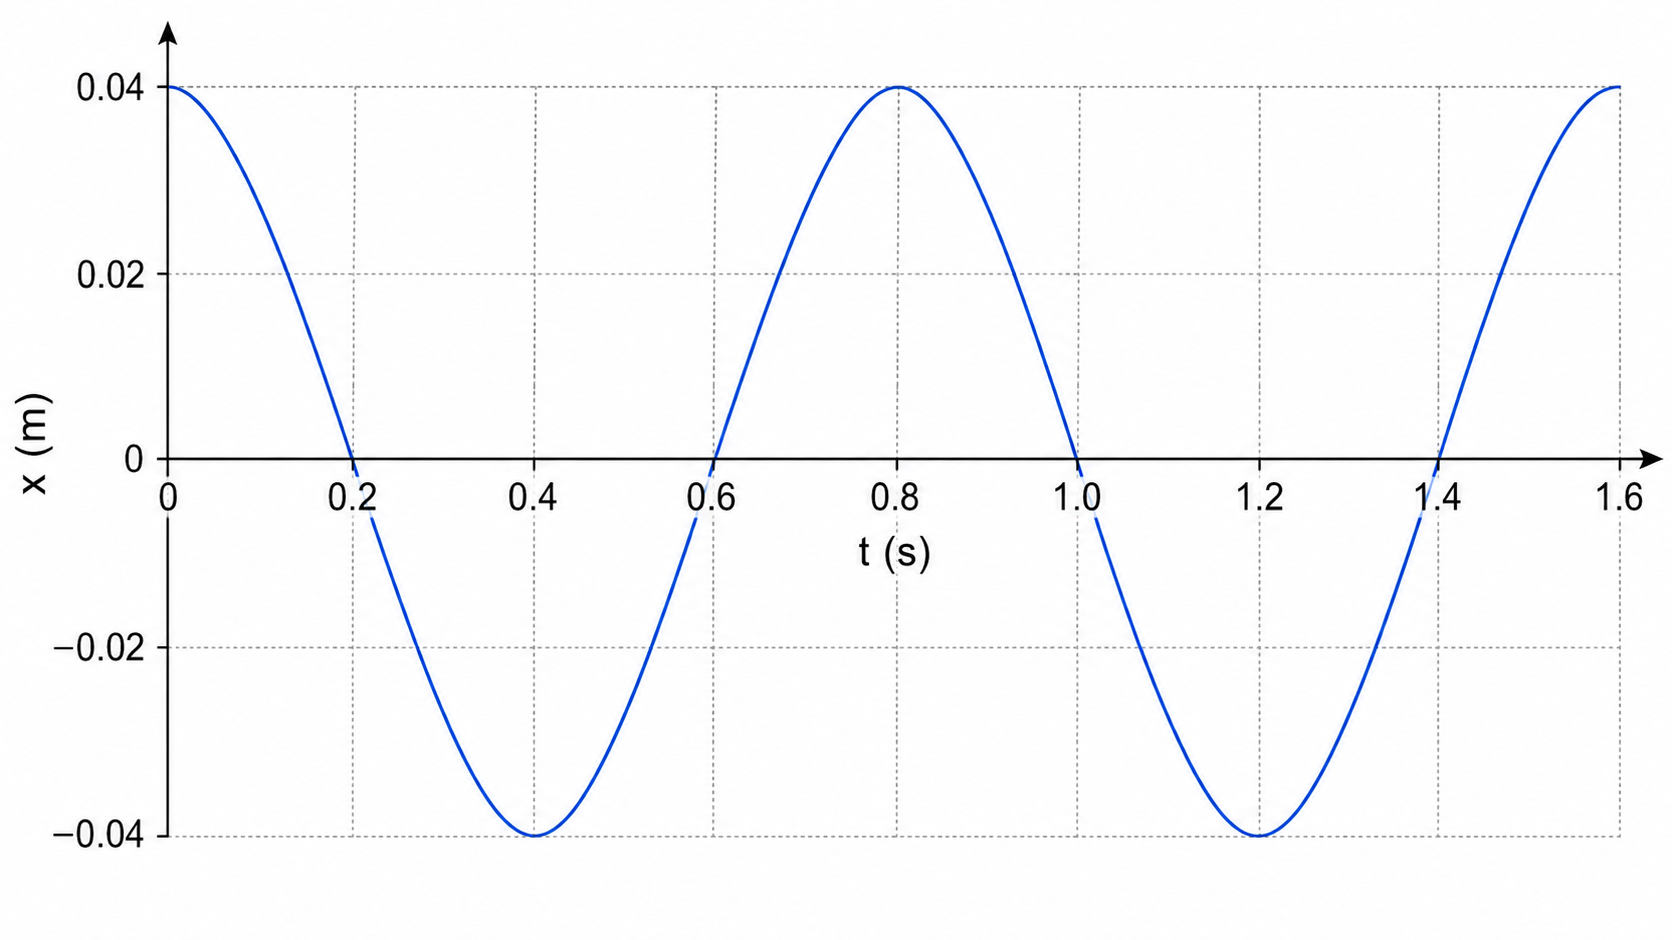
\includegraphics[width=0.8\textwidth]{graph1.png}
\caption{Displacement--time graph for Question 3}\label{fig:q3}
\end{figure}

A \SI{0.20}{kg} mass is attached to the spring.
\begin{enumerate}[label=(\alph*)]
\item From the graph, determine $A$ and $T$.
\item Hence find $\omega$ and write $x(t)$.
\item Calculate $v$ and $a$ at $t=\SI{0.30}{s}$.
\item Determine the spring constant $k$.
\end{enumerate}

\clearpage
\item \textbf{Graphical analysis II}\\
Figure~\ref{fig:q4} gives the velocity--time graph for a different SHM system.

\begin{figure}[h]
\centering
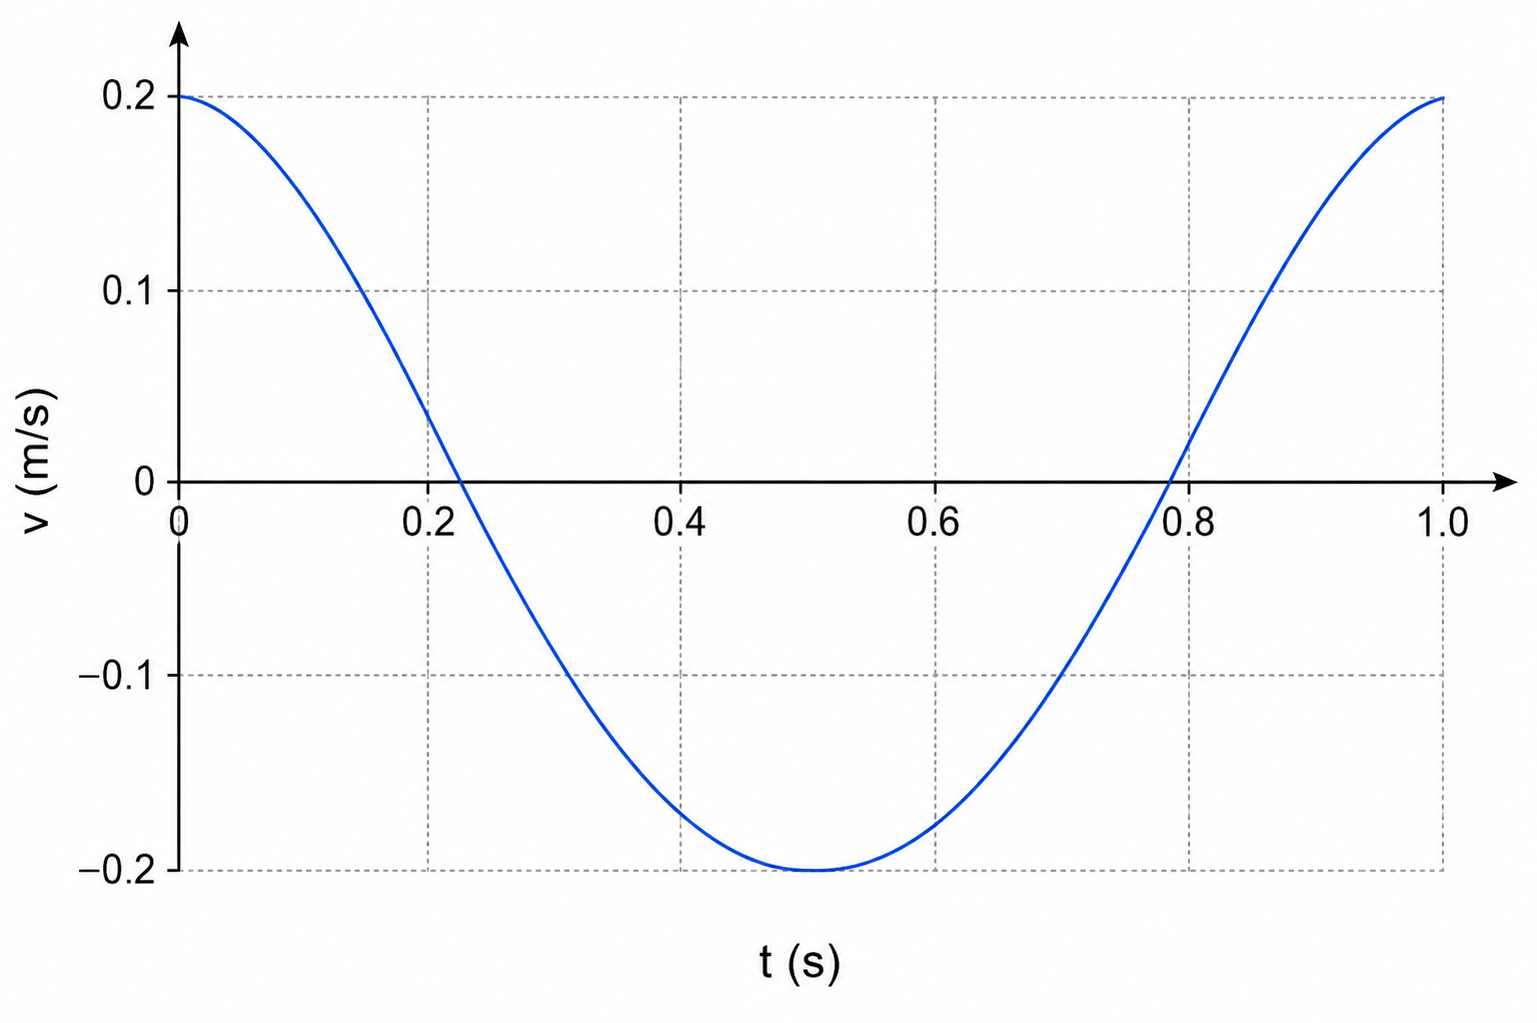
\includegraphics[width=0.8\textwidth]{graph2.png}
\caption{Velocity--time graph for Question 4}\label{fig:q4}
\end{figure}

\begin{enumerate}[label=(\alph*)]
\item Find the period and the velocity amplitude.
\item Deduce the displacement amplitude $A$.
\item Write expressions for $v(t)$ and $x(t)$.
\item When $v=\SI{0.15}{m\,s^{-1}}$ for the first time, calculate the displacement.
\end{enumerate}

\item \textbf{Vertical spring}\\
A \SI{0.20}{kg} mass hangs from a vertical spring. Pulling it down by \SI{0.050}{m} from the equilibrium position and releasing it initiates SHM. Ten complete oscillations take \SI{8.0}{s}.
\begin{enumerate}[label=(\alph*)]
\item Find $\omega$ and $k$.
\item Determine $v_\text{max}$ and $a_\text{max}$.
\item Calculate the total mechanical energy of the oscillation.
\end{enumerate}

\item \textbf{SHM quantities at a given displacement}\\
A \SI{0.40}{kg} block oscillates on a horizontal spring of force constant \SI{50}{N\,m^{-1}} with amplitude \SI{0.060}{m}.
\begin{enumerate}[label=(\alph*)]
\item Derive $v(x)$ and $a(x)$ for this system.
\item Calculate the speed and acceleration when $x=\SI{0.040}{m}$.
\item How long after passing equilibrium does the block first reach $x=\SI{0.040}{m}$?
\end{enumerate}
\end{enumerate}

\clearpage
\section*{Answer Key}
\begin{enumerate}[label=\textbf{Q\arabic*.}]
\item 
\begin{enumerate}[label=(\alph*)]
\item $\displaystyle x = 0.080\cos(6.98t)$
\item $v=-0.558\sin(6.98t),\quad a=-3.90\cos(6.98t)$
\item $v_\text{max}=0.558\;\text{m\,s}^{-1},\quad a_\text{max}=3.90\;\text{m\,s}^{-2}$
\item $k=m\omega^{2}=14.6\;\text{N\,m}^{-1}$
\item At $t=0.225$\,s: $x=0,\; v=-0.558$\,m\,s$^{-1},\; a=-3.90$\,m\,s$^{-2}$
\end{enumerate}

\item 
\begin{enumerate}[label=(\alph*)]
\item $A=0.099$\,m
\item $x=0.099\sin(4.04t),\; v=0.40\cos(4.04t)$
\item $t=0.050$\,s,\; $v=0.392$\,m\,s$^{-1}$
\item $a_\text{max}=1.62$\,m\,s$^{-2}$
\end{enumerate}

\item 
\begin{enumerate}[label=(\alph*)]
\item $A=0.040$\,m,\; $T=0.80$\,s
\item $\omega=7.85$\,rad\,s$^{-1},\; x=0.040\cos(7.85t)$
\item $x=-0.028$\,m,\; $v=-0.222$\,m\,s$^{-1}$,\; $a=1.75$\,m\,s$^{-2}$
\item $k=12.3$\,N\,m$^{-1}$
\end{enumerate}

\item 
\begin{enumerate}[label=(\alph*)]
\item $T=1.0$\,s,\; $v_\text{amp}=0.20$\,m\,s$^{-1}$
\item $A=0.032$\,m
\item $v=0.20\cos(6.28t),\; x=0.032\sin(6.28t)$
\item $x=0.021$\,m
\end{enumerate}

\item 
\begin{enumerate}[label=(\alph*)]
\item $\omega=7.85$\,rad\,s$^{-1}$,\; $k=12.3$\,N\,m$^{-1}$
\item $v_\text{max}=0.392$\,m\,s$^{-1}$,\; $a_\text{max}=3.09$\,m\,s$^{-2}$
\item $E=0.015$\,J
\end{enumerate}

\item 
\begin{enumerate}[label=(\alph*)]
\item $v(x)=\pm\omega\sqrt{A^{2}-x^{2}},\; a(x)=-\omega^{2}x$
\item $v=0.50$\,m\,s$^{-1}$,\; $a=-5.0$\,m\,s$^{-2}$
\item $t=0.065$\,s
\end{enumerate}
\end{enumerate}

\end{document}
